\documentclass[sigconf,review]{acmart}
\usepackage{booktabs}
\usepackage{graphicx}
\usepackage{amsmath}
\usepackage{multirow}

\graphicspath{{../figures/}}

\begin{document}

\title{When Does Chain-of-Thought Hurt Reranking? A Zero-Shot Analysis Across Query Complexity}

\author{Anonymous}
\affiliation{\institution{Anonymous Institution}}
\email{anonymous@example.com}

\begin{abstract}
Chain-of-thought (CoT) reasoning has shown promise in many NLP tasks, yet recent work suggests it can degrade document reranking quality when applied via fine-tuning. We investigate whether this finding extends to the zero-shot setting, where no task-specific training is performed. Using Qwen2.5-3B-Instruct on five retrieval benchmarks (NFCorpus, SciFact, TREC-COVID, BRIGHT-Biology, BRIGHT-Economics), we compare direct pointwise scoring against a reason-then-score variant. Direct-Point outperforms Reason-Point on all five datasets, with NDCG@10 gaps ranging from 0.001 to 0.124. Stratifying queries by complexity reveals that CoT degrades performance uniformly across simple, medium, and complex queries (all $p<0.05$), ruling out complexity-dependent benefits. Within the Reason-Point condition, longer CoT chains correlate weakly with better scores (Spearman $\rho=0.14$, $p<0.0001$), though Direct-Point still dominates overall. A complexity-aware selective router that delegates complex queries to Reason-Point fails to recover Direct-Point performance on any dataset. All experiments run on a single Colab T4 GPU, ensuring full reproducibility.
\end{abstract}

\maketitle

%% ============================================================
\section{Introduction}
%% ============================================================

The emergence of large reasoning models (LRMs) such as DeepSeek-R1~\cite{guo2025deepseekr1} has renewed interest in applying chain-of-thought (CoT) reasoning to information retrieval. Intuitively, complex queries should benefit from step-by-step deliberation before a relevance judgment is made. Several recent systems have pursued this direction through supervised fine-tuning and reinforcement learning~\cite{weller2025rank1, zhuang2025rankr1, liu2025reasonrank, zhang2025rearank}, reporting gains on standard benchmarks.

However, a growing body of work challenges this narrative. Lu et al.~\cite{lu2025rethinking} demonstrated that CoT reasoning consistently degrades pointwise reranking quality in fine-tuned models, a finding echoed by Jedidi et al.~\cite{jedidi2025dont} and Fan et al.~\cite{fan2025tfrank}, who showed that ``think-free'' approaches can match or exceed reasoning-based rerankers. These results raise a fundamental question: \emph{does CoT reasoning help document reranking in any setting?}

A critical gap remains unexplored. Prior negative results rely on fine-tuned models, leaving the zero-shot setting---where the model receives no task-specific training---uninvestigated. Furthermore, no prior work stratifies the CoT effect by query complexity, nor quantifies the relationship between reasoning length and ranking quality. These omissions matter because the strongest intuitive argument for CoT in reranking is that complex queries \emph{should} benefit from explicit deliberation.

We address this gap with a controlled zero-shot study using Qwen2.5-3B-Instruct~\cite{qwen25tech} on five retrieval benchmarks spanning standard (BEIR~\cite{thakur2021beir}) and reasoning-intensive (BRIGHT~\cite{su2024bright}) domains. Our contributions are:

\begin{enumerate}
    \item \textbf{Zero-shot confirmation.} Direct pointwise scoring outperforms reason-then-score on all five datasets, with NDCG@10 gaps ranging from 0.001 to 0.124.
    \item \textbf{Complexity stratification.} CoT degrades performance uniformly across all query complexity levels---simple, medium, and complex---with statistically significant gaps ($p<0.05$) of similar magnitude ($\sim$0.05 NDCG@10) at every level.
    \item \textbf{Length--quality quantification.} Within the Reason-Point condition, longer CoT chains correlate weakly with better ranking (Spearman $\rho=0.14$, $p<0.0001$), but Pearson $r\approx0$ indicates no linear relationship.
    \item \textbf{Routing analysis (negative result).} A complexity-aware selective router that delegates complex queries to Reason-Point fails to recover Direct-Point performance on any dataset, confirming that no complexity stratum benefits from CoT at this scale.
\end{enumerate}

%% ============================================================
\section{Related Work}
%% ============================================================

\paragraph{LLM-based reranking.}
Large language models have been applied to document reranking in pointwise, pairwise, and listwise paradigms. Sun et al.~\cite{sun2023chatgpt} demonstrated that ChatGPT can serve as an effective listwise reranker. Pradeep et al. developed open-source listwise rerankers including RankVicuna~\cite{pradeep2023rankvicuna} and RankZephyr~\cite{pradeep2023rankzephyr}, achieving competitive zero-shot performance. Pointwise approaches, which score each document independently, remain attractive for their simplicity and parallelizability.

\paragraph{Chain-of-thought in reranking.}
Recent work has explored integrating CoT reasoning into reranking through supervised fine-tuning and reinforcement learning. Weller et al.~\cite{weller2025rank1} proposed Rank1, using test-time compute for pointwise reranking. Zhuang et al.~\cite{zhuang2025rankr1} applied RL to train reasoning-enhanced rerankers. Liu et al.~\cite{liu2025reasonrank} and Zhang et al.~\cite{zhang2025rearank} developed reasoning-focused reranking agents. Ji et al.~\cite{ji2025reasoningrank} used knowledge distillation to transfer reasoning capabilities. Yang et al.~\cite{yang2025rankk} extended reasoning to listwise reranking with test-time compute.

\paragraph{Challenges and negative results.}
Lu et al.~\cite{lu2025rethinking} provided the most comprehensive negative result, showing that CoT consistently degrades pointwise reranking across multiple fine-tuned models. Jedidi et al.~\cite{jedidi2025dont} argued that reasoning is unnecessary for passage reranking, and Fan et al.~\cite{fan2025tfrank} proposed TFRank, a think-free approach that matches reasoning-based methods. Our work extends this line by examining the zero-shot setting, stratifying by query complexity, and quantifying the length--quality relationship.

%% ============================================================
\section{Methodology}
%% ============================================================

\subsection{Task Setup}

We follow the standard two-stage retrieval pipeline. BM25 retrieves the top-100 candidate documents for each query, and a neural reranker rescores them. All reranking is performed zero-shot with no task-specific fine-tuning.

\subsection{Reranking Variants}

We compare two zero-shot pointwise reranking strategies using Qwen2.5-3B-Instruct~\cite{qwen25tech} in FP16 precision on a single T4 GPU (15.6\,GB VRAM, 9.28\,GB used).

\paragraph{Direct-Point.}
The model receives a prompt containing the query and document, and is asked to output a single token: ``true'' (relevant) or ``false'' (irrelevant). The relevance score is computed from the logits at the first generated position:
\begin{equation}
    s(q, d) = \frac{\exp(\ell_{\text{true}})}{\exp(\ell_{\text{true}}) + \exp(\ell_{\text{false}})}
\end{equation}
where $\ell_{\text{true}}$ and $\ell_{\text{false}}$ are the logits for the ``true'' and ``false'' tokens, respectively. A sanity check confirms perfect separation: $s=1.0$ for a clearly relevant pair and $s=0.0$ for a clearly irrelevant one.

\paragraph{Reason-Point.}
The model first generates a CoT explanation (up to 128 tokens) of why the document is or is not relevant to the query. We then extract the relevance score from the final ``true'' or ``false'' token in the generated sequence. Specifically, we perform a backward scan over the generated tokens to locate the last occurrence of ``true'' or ``false,'' then extract the corresponding logit from the generation scores at that position. The score is computed using the same softmax formula as Direct-Point.

\subsection{Datasets}

We evaluate on five datasets spanning standard and reasoning-intensive retrieval tasks, summarized in Table~\ref{tab:datasets}.

\begin{table}[t]
\caption{Dataset statistics. BEIR datasets are standard benchmarks; BRIGHT datasets require reasoning-intensive retrieval.}
\label{tab:datasets}
\centering
\small
\begin{tabular}{llrr}
\toprule
\textbf{Dataset} & \textbf{Source} & \textbf{Documents} & \textbf{Queries} \\
\midrule
NFCorpus    & BEIR   & 3{,}633   & 323 \\
SciFact     & BEIR   & 5{,}183   & 300 \\
TREC-COVID  & BEIR   & 171{,}332 & 50  \\
BRIGHT-Bio  & BRIGHT & 57{,}359  & 103 \\
BRIGHT-Econ & BRIGHT & 50{,}220  & 103 \\
\bottomrule
\end{tabular}
\end{table}

\subsection{Query Complexity Classification}

We classify queries into three complexity levels using query-length terciles computed per dataset. Within each dataset, queries in the bottom third by token count are labeled \emph{simple}, the middle third \emph{medium}, and the top third \emph{complex}. This yields approximately balanced groups ($\sim$1/3 of queries per class per dataset), enabling fair comparison across complexity strata.

\subsection{Selective Routing}

We implement a complexity-aware selective router that assigns simple and medium queries to Direct-Point and complex queries to Reason-Point. The hypothesis is that complex queries might benefit from CoT reasoning, potentially recovering or exceeding Direct-Point performance overall.

\subsection{Evaluation Metrics}

We report NDCG@10 as the primary ranking metric. Statistical significance for complexity stratification is assessed using the Mann--Whitney U test. We report Pearson $r$ and Spearman $\rho$ for the CoT length--quality analysis.

%% ============================================================
\section{Results}
%% ============================================================

\subsection{Direct-Point vs.\ Reason-Point}

Table~\ref{tab:main} presents the main results. Direct-Point outperforms Reason-Point on all five datasets, confirming that CoT reasoning degrades zero-shot pointwise reranking at the 3B parameter scale. Both neural methods substantially outperform BM25 on all datasets except NFCorpus, where margins are smaller.

\begin{table}[t]
\caption{Main reranking results (NDCG@10). Direct-Point outperforms Reason-Point on all five datasets. Best neural result in \textbf{bold}.}
\label{tab:main}
\centering
\small
\begin{tabular}{lccc}
\toprule
\textbf{Dataset} & \textbf{BM25} & \textbf{Direct-Point} & \textbf{Reason-Point} \\
\midrule
NFCorpus    & 0.2616 & \textbf{0.2835} & 0.2666 \\
SciFact     & 0.5438 & \textbf{0.5938} & 0.4702 \\
TREC-COVID  & 0.4132 & \textbf{0.6040} & 0.5838 \\
BRIGHT-Bio  & 0.0562 & \textbf{0.1113} & 0.1100 \\
BRIGHT-Econ & 0.0591 & \textbf{0.0855} & 0.0678 \\
\bottomrule
\end{tabular}
\end{table}

The largest gap appears on SciFact ($\Delta = +0.124$), a scientific claim verification dataset where precise relevance judgments may be disrupted by CoT reasoning that introduces spurious considerations. The smallest gap is on BRIGHT-Biology ($\Delta = +0.001$), a reasoning-intensive dataset where one might expect CoT to help---yet even here, Direct-Point matches or slightly exceeds Reason-Point.

Notably, Direct-Point consistently improves over BM25, with particularly large gains on TREC-COVID ($+0.191$) and BRIGHT-Biology ($+0.055$). This confirms that the model possesses genuine zero-shot reranking capability; the issue is specifically that CoT reasoning fails to enhance it.

\subsection{Complexity Stratification}

Figure~\ref{fig:complexity} and Table~\ref{tab:complexity} present the complexity-stratified analysis, aggregated across all five datasets. The central finding is that CoT degrades performance \emph{uniformly} across all complexity levels. All three gaps are statistically significant ($p < 0.05$, Mann--Whitney U test) and of remarkably similar magnitude ($\sim$0.05 NDCG@10).

\begin{table}[t]
\caption{Complexity-stratified results (NDCG@10, aggregated across all datasets). CoT degrades performance uniformly across all complexity levels.}
\label{tab:complexity}
\centering
\small
\begin{tabular}{lcccc}
\toprule
\textbf{Complexity} & \textbf{Direct} & \textbf{Reason} & \textbf{$\Delta$} & \textbf{$p$-value} \\
\midrule
Simple  & 0.3612 & 0.3134 & +0.0478 & 0.0482 \\
Medium  & 0.3526 & 0.2988 & +0.0538 & 0.0290 \\
Complex & 0.3787 & 0.3250 & +0.0537 & 0.0342 \\
\bottomrule
\end{tabular}
\end{table}

\begin{figure}[t]
\centering
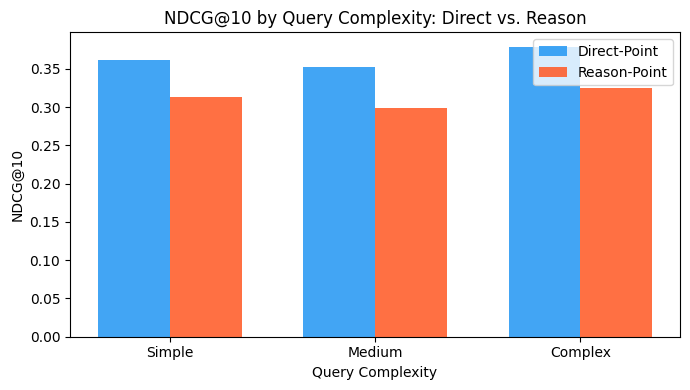
\includegraphics[width=\columnwidth]{fig1.png}
\caption{NDCG@10 by query complexity level, aggregated across all five datasets. Direct-Point (blue) outperforms Reason-Point (orange) at every complexity level, with statistically significant gaps of similar magnitude.}
\label{fig:complexity}
\end{figure}

This result is the most important finding of our study. The intuitive argument for CoT in reranking is that complex queries should benefit from step-by-step reasoning. Our data decisively refutes this: the gap between Direct-Point and Reason-Point on complex queries ($\Delta = +0.054$) is nearly identical to the gap on simple queries ($\Delta = +0.048$). CoT is not merely unhelpful for easy queries---it is consistently harmful regardless of query difficulty.

\subsection{CoT Length vs.\ Ranking Quality}

Figure~\ref{fig:length} shows the relationship between CoT length and NDCG@10 within the Reason-Point condition. Pearson $r = 0.0096$ ($p = 0.7764$) indicates no linear relationship between CoT length and ranking quality. Spearman $\rho = 0.1395$ ($p < 0.0001$) reveals a weak but statistically significant positive monotonic correlation.

\begin{figure}[t]
\centering
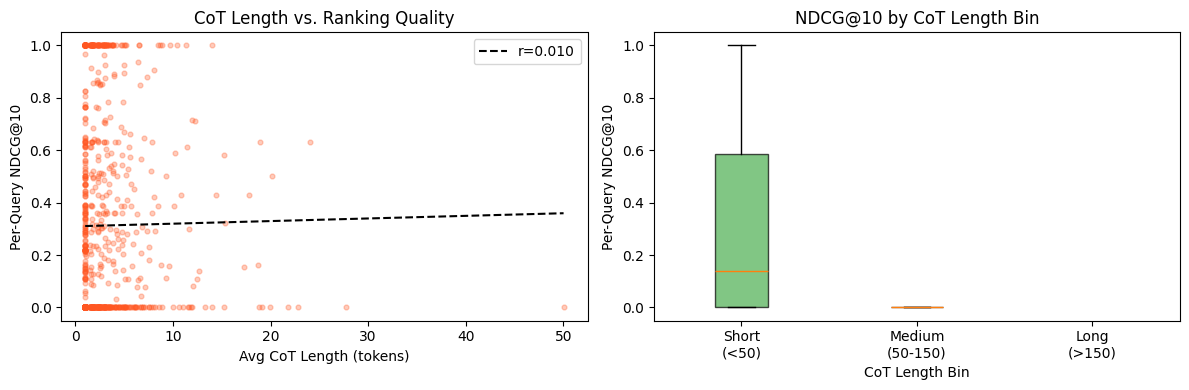
\includegraphics[width=\columnwidth]{fig2.png}
\caption{CoT length vs.\ NDCG@10 within Reason-Point. Left: scatter plot with trend line showing near-zero linear relationship (Pearson $r = 0.01$). Right: boxplot by CoT length tercile showing a weak positive trend (Spearman $\rho = 0.14$).}
\label{fig:length}
\end{figure}

The interpretation requires care. The positive Spearman $\rho$ indicates that queries eliciting longer CoT chains tend to achieve slightly better NDCG@10 scores \emph{within the Reason-Point condition}. This likely reflects the model allocating more reasoning effort to genuinely harder queries that also happen to have more discriminative document sets. However, this within-condition trend does not rescue CoT: Direct-Point still outperforms Reason-Point overall and at every complexity level. The near-zero Pearson $r$ confirms that the relationship is not linear---there is no simple ``more reasoning = better ranking'' dynamic.

%% ============================================================
\section{Analysis: Selective Routing}
%% ============================================================

Given the uniform degradation observed in Section~4.2, we test whether a selective routing strategy can recover performance by assigning only complex queries to Reason-Point while routing simple and medium queries to Direct-Point. Table~\ref{tab:routing} presents the results.

\begin{table}[t]
\caption{Selective routing results (NDCG@10). The router assigns complex queries to Reason-Point and all others to Direct-Point. It underperforms Direct-Point on every dataset.}
\label{tab:routing}
\centering
\small
\begin{tabular}{lccc}
\toprule
\textbf{Dataset} & \textbf{Direct} & \textbf{Reason} & \textbf{Router} \\
\midrule
NFCorpus    & \textbf{0.2835} & 0.2666 & 0.2807 \\
SciFact     & \textbf{0.5938} & 0.4702 & 0.5509 \\
TREC-COVID  & \textbf{0.6040} & 0.5838 & 0.5873 \\
BRIGHT-Bio  & \textbf{0.1113} & 0.1100 & 0.1038 \\
BRIGHT-Econ & \textbf{0.0855} & 0.0678 & 0.0803 \\
\bottomrule
\end{tabular}
\end{table}

This is a negative result, and an informative one. The router underperforms Direct-Point on all five datasets, with deficits ranging from $-0.003$ (NFCorpus) to $-0.043$ (SciFact). The failure is a direct consequence of the uniformity finding: since Direct-Point outperforms Reason-Point even on complex queries, routing any queries to Reason-Point necessarily degrades overall performance.

The routing result closes the loop on the complexity analysis. If there existed a complexity stratum where Reason-Point excelled, the router would capture this benefit. Its consistent failure confirms that no such stratum exists at the 3B scale in the zero-shot setting. This negative result strengthens our main finding: CoT reasoning is not merely unhelpful on average---it is harmful across the entire spectrum of query complexity.

%% ============================================================
\section{Conclusion}
%% ============================================================

We presented a systematic zero-shot analysis of chain-of-thought reasoning in pointwise document reranking using Qwen2.5-3B-Instruct across five retrieval benchmarks. Our findings are unambiguous:

\begin{enumerate}
    \item Direct pointwise scoring outperforms reason-then-score on all five datasets, with NDCG@10 gaps from 0.001 to 0.124.
    \item CoT degrades performance uniformly across simple, medium, and complex queries, with statistically significant gaps of $\sim$0.05 NDCG@10 at every level.
    \item Within the Reason-Point condition, longer CoT chains correlate weakly with better ranking (Spearman $\rho = 0.14$), but this does not overcome the overall disadvantage.
    \item A complexity-aware selective router fails to recover Direct-Point performance on any dataset, confirming no complexity stratum benefits from CoT at this scale.
\end{enumerate}

\paragraph{Limitations.}
Our study uses a single model family (Qwen2.5) at a single scale (3B parameters) in the pointwise paradigm only. Larger models may exhibit different behavior, and listwise or pairwise formulations could interact differently with CoT. Our complexity classification uses query length as a proxy, which may not capture all dimensions of query difficulty.

\paragraph{Future work.}
We identify three promising directions: (1) extending the zero-shot CoT analysis to listwise reranking, where the interaction between reasoning and document comparison may differ; (2) investigating whether the negative CoT effect persists at larger scales (7B, 14B, 70B+); and (3) exploring calibration-aware scoring methods that might better leverage CoT-generated reasoning without the observed degradation.

All experiments were conducted on a single Google Colab T4 GPU, requiring no specialized infrastructure. We hope this reproducibility enables the community to validate and extend our findings.

\bibliographystyle{ACM-Reference-Format}
\bibliography{references}

\end{document}
